% Options for packages loaded elsewhere
\PassOptionsToPackage{unicode}{hyperref}
\PassOptionsToPackage{hyphens}{url}
\PassOptionsToPackage{dvipsnames,svgnames,x11names}{xcolor}
%
\documentclass[
  letterpaper,
  DIV=11,
  numbers=noendperiod]{scrartcl}

\usepackage{amsmath,amssymb}
\usepackage{iftex}
\ifPDFTeX
  \usepackage[T1]{fontenc}
  \usepackage[utf8]{inputenc}
  \usepackage{textcomp} % provide euro and other symbols
\else % if luatex or xetex
  \usepackage{unicode-math}
  \defaultfontfeatures{Scale=MatchLowercase}
  \defaultfontfeatures[\rmfamily]{Ligatures=TeX,Scale=1}
\fi
\usepackage{lmodern}
\ifPDFTeX\else  
    % xetex/luatex font selection
\fi
% Use upquote if available, for straight quotes in verbatim environments
\IfFileExists{upquote.sty}{\usepackage{upquote}}{}
\IfFileExists{microtype.sty}{% use microtype if available
  \usepackage[]{microtype}
  \UseMicrotypeSet[protrusion]{basicmath} % disable protrusion for tt fonts
}{}
\makeatletter
\@ifundefined{KOMAClassName}{% if non-KOMA class
  \IfFileExists{parskip.sty}{%
    \usepackage{parskip}
  }{% else
    \setlength{\parindent}{0pt}
    \setlength{\parskip}{6pt plus 2pt minus 1pt}}
}{% if KOMA class
  \KOMAoptions{parskip=half}}
\makeatother
\usepackage{xcolor}
\setlength{\emergencystretch}{3em} % prevent overfull lines
\setcounter{secnumdepth}{-\maxdimen} % remove section numbering
% Make \paragraph and \subparagraph free-standing
\ifx\paragraph\undefined\else
  \let\oldparagraph\paragraph
  \renewcommand{\paragraph}[1]{\oldparagraph{#1}\mbox{}}
\fi
\ifx\subparagraph\undefined\else
  \let\oldsubparagraph\subparagraph
  \renewcommand{\subparagraph}[1]{\oldsubparagraph{#1}\mbox{}}
\fi

\usepackage{color}
\usepackage{fancyvrb}
\newcommand{\VerbBar}{|}
\newcommand{\VERB}{\Verb[commandchars=\\\{\}]}
\DefineVerbatimEnvironment{Highlighting}{Verbatim}{commandchars=\\\{\}}
% Add ',fontsize=\small' for more characters per line
\usepackage{framed}
\definecolor{shadecolor}{RGB}{241,243,245}
\newenvironment{Shaded}{\begin{snugshade}}{\end{snugshade}}
\newcommand{\AlertTok}[1]{\textcolor[rgb]{0.68,0.00,0.00}{#1}}
\newcommand{\AnnotationTok}[1]{\textcolor[rgb]{0.37,0.37,0.37}{#1}}
\newcommand{\AttributeTok}[1]{\textcolor[rgb]{0.40,0.45,0.13}{#1}}
\newcommand{\BaseNTok}[1]{\textcolor[rgb]{0.68,0.00,0.00}{#1}}
\newcommand{\BuiltInTok}[1]{\textcolor[rgb]{0.00,0.23,0.31}{#1}}
\newcommand{\CharTok}[1]{\textcolor[rgb]{0.13,0.47,0.30}{#1}}
\newcommand{\CommentTok}[1]{\textcolor[rgb]{0.37,0.37,0.37}{#1}}
\newcommand{\CommentVarTok}[1]{\textcolor[rgb]{0.37,0.37,0.37}{\textit{#1}}}
\newcommand{\ConstantTok}[1]{\textcolor[rgb]{0.56,0.35,0.01}{#1}}
\newcommand{\ControlFlowTok}[1]{\textcolor[rgb]{0.00,0.23,0.31}{#1}}
\newcommand{\DataTypeTok}[1]{\textcolor[rgb]{0.68,0.00,0.00}{#1}}
\newcommand{\DecValTok}[1]{\textcolor[rgb]{0.68,0.00,0.00}{#1}}
\newcommand{\DocumentationTok}[1]{\textcolor[rgb]{0.37,0.37,0.37}{\textit{#1}}}
\newcommand{\ErrorTok}[1]{\textcolor[rgb]{0.68,0.00,0.00}{#1}}
\newcommand{\ExtensionTok}[1]{\textcolor[rgb]{0.00,0.23,0.31}{#1}}
\newcommand{\FloatTok}[1]{\textcolor[rgb]{0.68,0.00,0.00}{#1}}
\newcommand{\FunctionTok}[1]{\textcolor[rgb]{0.28,0.35,0.67}{#1}}
\newcommand{\ImportTok}[1]{\textcolor[rgb]{0.00,0.46,0.62}{#1}}
\newcommand{\InformationTok}[1]{\textcolor[rgb]{0.37,0.37,0.37}{#1}}
\newcommand{\KeywordTok}[1]{\textcolor[rgb]{0.00,0.23,0.31}{#1}}
\newcommand{\NormalTok}[1]{\textcolor[rgb]{0.00,0.23,0.31}{#1}}
\newcommand{\OperatorTok}[1]{\textcolor[rgb]{0.37,0.37,0.37}{#1}}
\newcommand{\OtherTok}[1]{\textcolor[rgb]{0.00,0.23,0.31}{#1}}
\newcommand{\PreprocessorTok}[1]{\textcolor[rgb]{0.68,0.00,0.00}{#1}}
\newcommand{\RegionMarkerTok}[1]{\textcolor[rgb]{0.00,0.23,0.31}{#1}}
\newcommand{\SpecialCharTok}[1]{\textcolor[rgb]{0.37,0.37,0.37}{#1}}
\newcommand{\SpecialStringTok}[1]{\textcolor[rgb]{0.13,0.47,0.30}{#1}}
\newcommand{\StringTok}[1]{\textcolor[rgb]{0.13,0.47,0.30}{#1}}
\newcommand{\VariableTok}[1]{\textcolor[rgb]{0.07,0.07,0.07}{#1}}
\newcommand{\VerbatimStringTok}[1]{\textcolor[rgb]{0.13,0.47,0.30}{#1}}
\newcommand{\WarningTok}[1]{\textcolor[rgb]{0.37,0.37,0.37}{\textit{#1}}}

\providecommand{\tightlist}{%
  \setlength{\itemsep}{0pt}\setlength{\parskip}{0pt}}\usepackage{longtable,booktabs,array}
\usepackage{calc} % for calculating minipage widths
% Correct order of tables after \paragraph or \subparagraph
\usepackage{etoolbox}
\makeatletter
\patchcmd\longtable{\par}{\if@noskipsec\mbox{}\fi\par}{}{}
\makeatother
% Allow footnotes in longtable head/foot
\IfFileExists{footnotehyper.sty}{\usepackage{footnotehyper}}{\usepackage{footnote}}
\makesavenoteenv{longtable}
\usepackage{graphicx}
\makeatletter
\def\maxwidth{\ifdim\Gin@nat@width>\linewidth\linewidth\else\Gin@nat@width\fi}
\def\maxheight{\ifdim\Gin@nat@height>\textheight\textheight\else\Gin@nat@height\fi}
\makeatother
% Scale images if necessary, so that they will not overflow the page
% margins by default, and it is still possible to overwrite the defaults
% using explicit options in \includegraphics[width, height, ...]{}
\setkeys{Gin}{width=\maxwidth,height=\maxheight,keepaspectratio}
% Set default figure placement to htbp
\makeatletter
\def\fps@figure{htbp}
\makeatother

\KOMAoption{captions}{tableheading}
\makeatletter
\makeatother
\makeatletter
\makeatother
\makeatletter
\@ifpackageloaded{caption}{}{\usepackage{caption}}
\AtBeginDocument{%
\ifdefined\contentsname
  \renewcommand*\contentsname{Table of contents}
\else
  \newcommand\contentsname{Table of contents}
\fi
\ifdefined\listfigurename
  \renewcommand*\listfigurename{List of Figures}
\else
  \newcommand\listfigurename{List of Figures}
\fi
\ifdefined\listtablename
  \renewcommand*\listtablename{List of Tables}
\else
  \newcommand\listtablename{List of Tables}
\fi
\ifdefined\figurename
  \renewcommand*\figurename{Figure}
\else
  \newcommand\figurename{Figure}
\fi
\ifdefined\tablename
  \renewcommand*\tablename{Table}
\else
  \newcommand\tablename{Table}
\fi
}
\@ifpackageloaded{float}{}{\usepackage{float}}
\floatstyle{ruled}
\@ifundefined{c@chapter}{\newfloat{codelisting}{h}{lop}}{\newfloat{codelisting}{h}{lop}[chapter]}
\floatname{codelisting}{Listing}
\newcommand*\listoflistings{\listof{codelisting}{List of Listings}}
\makeatother
\makeatletter
\@ifpackageloaded{caption}{}{\usepackage{caption}}
\@ifpackageloaded{subcaption}{}{\usepackage{subcaption}}
\makeatother
\makeatletter
\@ifpackageloaded{tcolorbox}{}{\usepackage[skins,breakable]{tcolorbox}}
\makeatother
\makeatletter
\@ifundefined{shadecolor}{\definecolor{shadecolor}{rgb}{.97, .97, .97}}
\makeatother
\makeatletter
\makeatother
\makeatletter
\makeatother
\ifLuaTeX
  \usepackage{selnolig}  % disable illegal ligatures
\fi
\IfFileExists{bookmark.sty}{\usepackage{bookmark}}{\usepackage{hyperref}}
\IfFileExists{xurl.sty}{\usepackage{xurl}}{} % add URL line breaks if available
\urlstyle{same} % disable monospaced font for URLs
\hypersetup{
  pdftitle={Linear Regression Tutorial},
  colorlinks=true,
  linkcolor={blue},
  filecolor={Maroon},
  citecolor={Blue},
  urlcolor={Blue},
  pdfcreator={LaTeX via pandoc}}

\title{Linear Regression Tutorial}
\author{}
\date{}

\begin{document}
\maketitle
\ifdefined\Shaded\renewenvironment{Shaded}{\begin{tcolorbox}[frame hidden, borderline west={3pt}{0pt}{shadecolor}, interior hidden, boxrule=0pt, enhanced, sharp corners, breakable]}{\end{tcolorbox}}\fi

\begin{center}\rule{0.5\linewidth}{0.5pt}\end{center}

In this tutorial you will perform a linear regression and make the
machine learn.\\
Now, to run a code block in Jupyter Notebooks, click into it and hit
ctrl + enter.\\
If the key command doesn't work, hit the triangle button in the upper
left.\\
The first step, of course, is to load the data. We will be using a
dataset of shampoo sales over 3 years.

\begin{Shaded}
\begin{Highlighting}[]
\ImportTok{import}\NormalTok{ csv}
\ImportTok{import}\NormalTok{ datetime }\ImportTok{as}\NormalTok{ dt}

\ControlFlowTok{with} \BuiltInTok{open}\NormalTok{(}\StringTok{"shampoo.csv"}\NormalTok{, }\StringTok{"r"}\NormalTok{) }\ImportTok{as}\NormalTok{ shamwow:}
\NormalTok{    data }\OperatorTok{=} \BuiltInTok{list}\NormalTok{(csv.reader(shamwow))[}\DecValTok{1}\NormalTok{:]}

\CommentTok{\# Convert the sales into a float}
\NormalTok{sales }\OperatorTok{=}\NormalTok{ [}\BuiltInTok{float}\NormalTok{(point[}\DecValTok{1}\NormalTok{]) }\ControlFlowTok{for}\NormalTok{ point }\KeywordTok{in}\NormalTok{ data]}
\NormalTok{dates }\OperatorTok{=}\NormalTok{ [dt.datetime.strptime(}\StringTok{"199"} \OperatorTok{+}\NormalTok{ point[}\DecValTok{0}\NormalTok{],}\StringTok{\textquotesingle{}\%Y{-}\%m\textquotesingle{}}\NormalTok{).date() }
         \ControlFlowTok{for}\NormalTok{ point }\KeywordTok{in}\NormalTok{ data]}

\BuiltInTok{print}\NormalTok{(sales[}\DecValTok{0}\NormalTok{:}\DecValTok{5}\NormalTok{])}
\BuiltInTok{print}\NormalTok{(dates[}\DecValTok{0}\NormalTok{:}\DecValTok{2}\NormalTok{])}
\end{Highlighting}
\end{Shaded}

\begin{verbatim}
[266.0, 145.9, 183.1, 119.3, 180.3]
[datetime.date(1991, 1, 1), datetime.date(1991, 2, 1)]
\end{verbatim}

Let's plot the data in a plot that's as scattered as my brain while
writing this tutorial:

\begin{Shaded}
\begin{Highlighting}[]
\ImportTok{import}\NormalTok{ matplotlib.pyplot }\ImportTok{as}\NormalTok{ plt}
\ImportTok{import}\NormalTok{ matplotlib.dates }\ImportTok{as}\NormalTok{ mdates}

\CommentTok{\# Format X{-}axis properly}
\NormalTok{plt.gca().xaxis.set\_major\_formatter(mdates.DateFormatter(}\StringTok{\textquotesingle{}\%m/\%Y\textquotesingle{}}\NormalTok{))}
\NormalTok{plt.gca().xaxis.set\_major\_locator(mdates.MonthLocator(interval}\OperatorTok{=}\DecValTok{5}\NormalTok{))}
\NormalTok{plt.gcf().autofmt\_xdate()}

\CommentTok{\# Plot with X{-}axis as date and Y{-}axis as sales}
\NormalTok{points }\OperatorTok{=}\NormalTok{ plt.scatter(d)}
\end{Highlighting}
\end{Shaded}

\begin{figure}[H]

{\centering 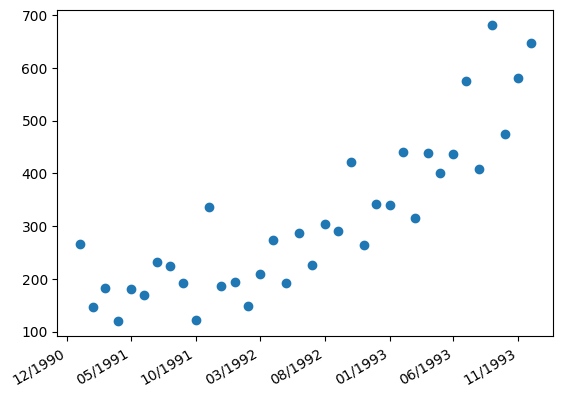
\includegraphics{00_core_files/figure-pdf/cell-3-output-1.png}

}

\end{figure}

Now let's perform the actual linear regression. We're fitting the data
to a line. What degree polynomial does that correspond to? Hopefully I
have at least that many degrees by the time I leave college\ldots{}

\begin{Shaded}
\begin{Highlighting}[]
\ImportTok{import}\NormalTok{ numpy }\ImportTok{as}\NormalTok{ np}

\CommentTok{\# Converting the datetime objects into an integer}
\NormalTok{counter }\OperatorTok{=} \DecValTok{1}
\NormalTok{numeric\_months }\OperatorTok{=}\NormalTok{ []}
\ControlFlowTok{for}\NormalTok{ date }\KeywordTok{in}\NormalTok{ dates:}
\NormalTok{    numeric\_months.append(counter)}
\NormalTok{    counter }\OperatorTok{+=} \DecValTok{1}

\CommentTok{\# Linear regression using a polynomial of a certain degree}
\NormalTok{linear\_regression }\OperatorTok{=}\NormalTok{ np.polyfit(numeric\_months, sales, }\DecValTok{1}\NormalTok{)}
\end{Highlighting}
\end{Shaded}

Remember like 5 years ago when you learned about slope-intercept form?
Y'know, y = mx + b where m is the slope and b is the y-intercept? Don't
ask me why I still remember that, but we're gonna use it now to plot the
linear regression line:

\begin{Shaded}
\begin{Highlighting}[]
\ImportTok{import}\NormalTok{ matplotlib.ticker }\ImportTok{as}\NormalTok{ ticker}

\NormalTok{m, b }\OperatorTok{=}\NormalTok{ linear\_regression}

\CommentTok{\# Replicate the same formatting as the dates}
\NormalTok{formatted\_dates }\OperatorTok{=}\NormalTok{ [date.strftime(}\StringTok{\textquotesingle{}\%m/\%Y\textquotesingle{}}\NormalTok{) }\ControlFlowTok{for}\NormalTok{ date }\KeywordTok{in}\NormalTok{ dates]}
\NormalTok{formatted\_dates.insert(}\DecValTok{0}\NormalTok{, }\StringTok{"12/1990"}\NormalTok{)}
\NormalTok{ticks }\OperatorTok{=}\NormalTok{ [}\DecValTok{0}\NormalTok{] }\OperatorTok{+}\NormalTok{ numeric\_months}

\CommentTok{\# Plot with X{-}axis as dates}
\NormalTok{plt.gca().set\_xticks(ticks, formatted\_dates)}
\NormalTok{plt.gcf().autofmt\_xdate()}
\NormalTok{plt.gca().xaxis.set\_major\_locator(ticker.MultipleLocator(}\DecValTok{5}\NormalTok{))}
\NormalTok{points }\OperatorTok{=}\NormalTok{ plt.scatter(numeric\_months, sales)}

\CommentTok{\# One of them is the Y{-}intercept, and one of them is slope}
\NormalTok{line }\OperatorTok{=}\NormalTok{ plt.axline((}\DecValTok{0}\NormalTok{, ?), slope}\OperatorTok{=}\NormalTok{?, color}\OperatorTok{=}\StringTok{"red"}\NormalTok{)}
\end{Highlighting}
\end{Shaded}

\begin{figure}[H]

{\centering 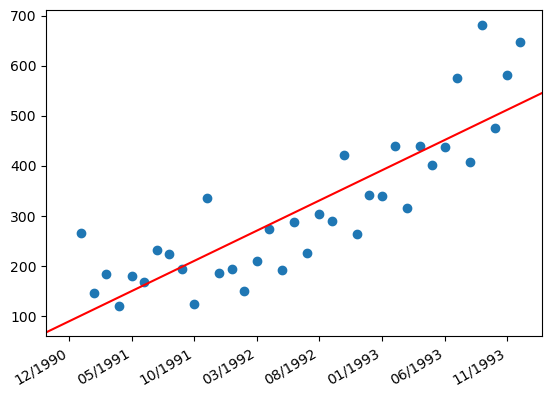
\includegraphics{00_core_files/figure-pdf/cell-5-output-1.png}

}

\end{figure}

Congratulations, you did it! Now go to the upper left corner, hit file,
press new, open a terminal, get to the right directory, and type\\
\texttt{quarto\ render\ 00\_core.ipynb\ -\/-to\ docx}

Then, simply convert it to a PDF and email it to Alejandro and CC
Prof.~Poshyvanyk!

References:\\
Where I found the shampoo data:
https://machinelearningmastery.com/time-series-datasets-for-machine-learning/\\
Original Source: Makridakis, S., Wheelwright, S.C. and Hyndman, R.J.
(1998) Forecasting: Methods and Applications. 3rd Edition, Wiley, New
York.



\end{document}
